\RCS$Revision: 230053 $
\RCS$HeadURL: svn+ssh://svn.cern.ch/reps/tdr2/notes/AN-14-062/trunk/AN-14-062.tex $
\RCS$Id: AN-14-062.tex 230053 2014-03-05 06:58:25Z syu $
%%%%%%%%%%%%% local definitions %%%%%%%%%%%%%%%%%%%%%
% This allows for switching between one column and two column (cms@external) layouts
% The widths should  be modified for your particular figures. You'll need additional copies if you have more than one standard figure size.
\newlength\cmsFigWidth
\ifthenelse{\boolean{cms@external}}{\setlength\cmsFigWidth{0.85\columnwidth}}{\setlength\cmsFigWidth{0.4\textwidth}}
\ifthenelse{\boolean{cms@external}}{\providecommand{\cmsLeft}{top}}{\providecommand{\cmsLeft}{left}}
\ifthenelse{\boolean{cms@external}}{\providecommand{\cmsRight}{bottom}}{\providecommand{\cmsRight}{right}}
%%%%%%%%%%%%%%%  Title page %%%%%%%%%%%%%%%%%%%%%%%%
\cmsNoteHeader{MOST 104-2112-M-008-015-MY3} % This is over-written in the CMS environment: useful as preprint no. for export versions

% >> Title: please make sure that the non-TeX equivalent is in PDFTitle below
\title{Midterm Report (2015/08/01--2016/07/31): \bf{MOST 104-2112-M-008-015-MY3}}

% >> Authors
%Author is always "The CMS Collaboration" for PAS and papers, so author, etc, below will be ignored in those cases
%For multiple affiliations, create an address entry for the combination
%To mark authors as primary, use the \author* form
\address[NCU]{National Central University,  Chung-Li, Taiwan}
\author[NCU]{Shin-Shan Yu}


% >> Date
% The date is in yyyy/mm/dd format. Today has been
% redefined to match, but if the date needs to be fixed, please write it in this fashion.
% For papers and PAS, \today is taken as the date the head file (this one) was last modified according to svn: see the RCS Id string above.
% For the final version it is best to "touch" the head file to make sure it has the latest date.

% >> Abstract
% Abstract processing:
% 1. **DO NOT use \include or \input** to include the abstract: our abstract extractor will not search through other files than this one.
% 2. **DO NOT use %**                  to comment out sections of the abstract: the extractor will still grab those lines (and they won't be comments any longer!).
% 3. For PASs: **DO NOT use tex macros**         in the abstract: CDS MathJax processor used on the abstract doesn't understand them _and_ will only look within $$. The abstracts for papers are hand formatted so macros are okay.
\abstract{We have joined the CMS phase-II upgrade project HGC. At this moment, we have completed the sensor designs and the mask productions. The manufacturing company, APM, is expected to deliver the first batch in late July of 2016. Meanwhile, we will join the test beam effort at the CERN H2 beam line.
}


% >> PDF Metadata
% Do not comment out the following hypersetup lines (metadata). They will disappear in NODRAFT mode and are needed by CDS.
% Also: make sure that the values of the metadata items are sensible and are in plain text:
% (1) no TeX! -- for \sqrt{s} use sqrt(s) -- this will show with extra quote marks in the draft version but is okay).
% (2) no %.
% (3) No curly braces {}.
\hypersetup{%
pdfauthor={Shin-Shan Yu},%
pdftitle={Midterm Report},%
pdfsubject={CMS},%
pdfkeywords={LHC, CMS, phase 2 detector upgrade, high granularity calorimeter, mask}
}

\maketitle %maketitle comes after all the front information has been
Note, the talk of HGC test beam analysis by Yu-hsiang Chang is attached at the end of this report.

\section{Status of the Sensor R\&D at NCU}
The manpower working on the sensor R\&D at NCU is Prof. Willis Lin, the 
assistants Hilary Chang and Fang-Ying Tsai. 

The major task of High Granularity Calorimeter (HGC) is to replace the 
CMS endcap calorimeters. More details of the HGC design and expected 
performance could be found in the CMS Technical Proposal~\cite{HGC-TDR}. 
In order to improve the position resolution, the HGC geometry is a hexagonal 
cells combination. Each hexagon is about 1~centimeter square. 

At this stage, we concentrate on sensor processing as followings.
\begin{enumerate}
\item Starting from sensor cleaning
\item Gettering
\item Front-side cap
\item Backside n$^{+}$ implantation
\item Apply first mask and remove Si$_2$N$_3$
\item Front side p$^{+}$ implantation
\item Driving in and oxidation
\item Apply second mask, define contact holes
\item Metal deposition
\item Apply third mask to define metal patterns
\item Passivation deposition
\item Apply fourth mask to define the metal contact
\item Backside metal deposition an anneal
\end{enumerate}

The Asia Pacific Micron tech, APM, will deliver the first pilot run by
the end of July 2016. See the attached slides for the issues of the backside 
of sensors.

\section{Analysis of the HGC Test Beam Data}
The manpower working on the test beam data includes Prof. Shin-Shan Yu, the postdoc Dr. Vieri Candelise, and the 
Ph.D. student Yu-Hsiang Chang. We collaborated with a CERN postdoc Arabella Martelli and studied the correlation 
between the peak of the readout signal and the input amount of charge (integrated from -40 to +50 ps around the 
peak). After requiring the peak to be greater than 150 ADC counts and requiring that the signal to be within the 
fiducial region, we find a nice correlation between the peak and the integrated charge. The only exception is 
the channel that is known to be bad.
See Fig.~\ref{fig:testbeam_analysis} for the correlation of all the channels we studied.

\begin{figure}[htbp]
   \centering
   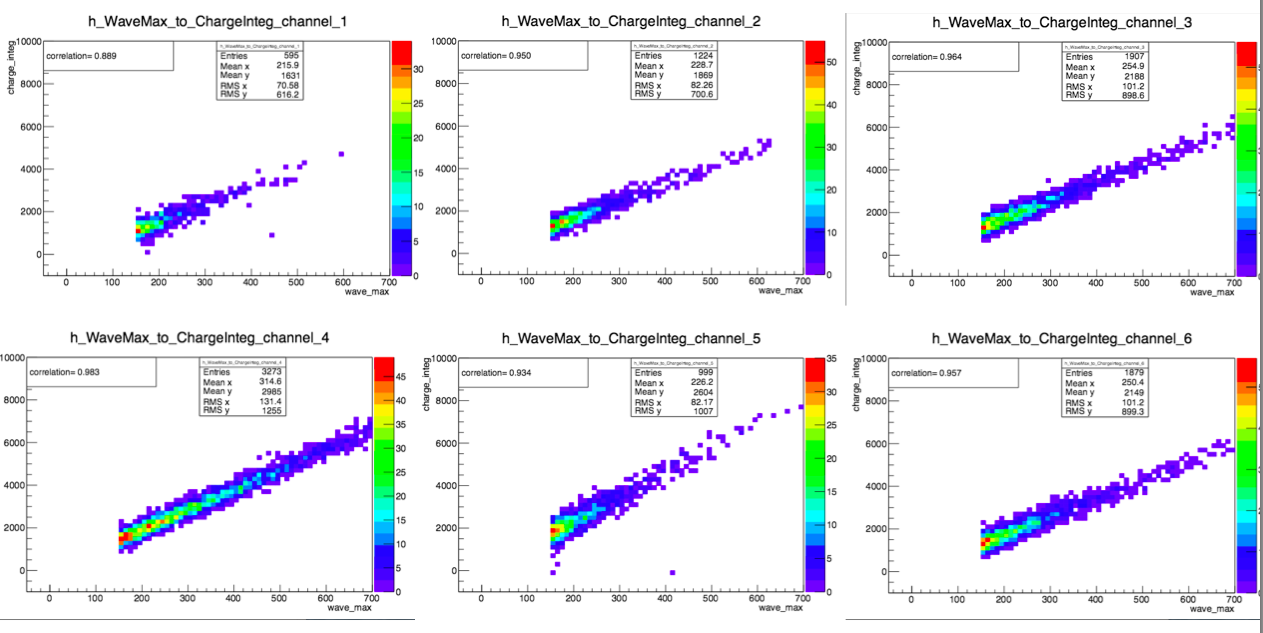
\includegraphics[width=0.9\textwidth]{figures/testbeam_analysis.png}
   \caption{The 2-D distributions of integrated amount of charge vs. the peak value of the signal for all readout channels.}
   \label{fig:testbeam_analysis}
\end{figure}




\bibliography{auto_generated}

